% %%%%%%%%%%%%%%%%%%%%%%%%%%%%%%%%%%%%%%%%%%%%%%%%%%%%%%%%%%%%%%%%%%%%%
% %% State-of-the-Art %%
% Accelerators Comparison
% %%%%%%%%%%%%%%%%%%%%%%%%%%%%%%%%%%%%%%%%%%%%%%%%%%%%%%%%%%%%%%%%%%%%%

\section{Comparison of Existing Accelerators}
\label{sec:soa:comparison_and_analysis}

In this section, we analyze and further compare the accelerators that were described in Section~\ref{sec:soa:hw_accelerators}. We start with Table~\ref{tab:soa:classificationMaturity} where we summarize the accelerators, chronologically, showing the research group where they were developed. We see that MIT is very active in the field, as they were involved in developing four different accelerators (\emph{e.g.} ExTensor, PHI, SpArch and Gamma).

\begin{table}
    \caption{Chronological Summary of Sparse Accelerators}
    \centering
    \footnotesize
    \begin{tabular}{|c|c|| >{\centering\arraybackslash}m{4.05cm}|| >{\centering\arraybackslash}m{7.19cm}|}
        \hhline{--||-||-}
        \textbf{Name} & \textbf{Date} & \textbf{Institute / University} & \textbf{Summary} \\
        \hhline{==::=::=}
        OuterSPACE~\cite{Pal2018_OuterSPACE} & 2018 & Univ. of Michigan / Arizona State Univ. & Highly parallelized SPMD, two levels cache -- \algo{OP} SpMSpM \\
        \hhline{--||-||-}
        ExTensor~\cite{Hegde2019_ExTensor} & 2019 & Univ. of Illinois / NVIDIA / MIT & General purpose tensor algebra -- With \emph{tiled} SpMSpM \\
        \hhline{--||-||-}
        PHI~\cite{Mukkara2019_PHI} & 2019 & MIT (CSAIL) / Carnegie Mellon Univ. & In cache, hash-based accelerator for \emph{reductions} \\
        \hhline{--||-||-}
        SPiDRE~\cite{Barredo2019_SPiDRE} & 2019 & UPC, BSC (Spain) / Arm Research & Near main memory data reorganisation for \emph{intersections} \\
        \hhline{--||-||-}
        MatRaptor~\cite{Srivastava2020_MatRaptor} & 2020 & Cornell & Row-parallel with HBM-aware custom format -- \algo{Gust} SpMSpM \\
        \hhline{--||-||-}
        SpArch~\cite{Zhekai2020_SpArch} & 2020 & MIT / Stanford / NVIDIA & Compression method to reduce \emph{POs}, \emph{multiply}/\emph{merge} pipe -- \algo{OP} SpGEMM \\
        \hhline{--||-||-}
        SpaceA~\cite{Xie2021_SpaceA} & 2021 & UC Santa Barbara & In memory accelerator for 3D DRAM -- \algo{IP} SpMV \\
        \hhline{--||-||-}
        Gamma~\cite{Zhang2021_Gamma} & 2021 & MIT (CSAIL) & Parallelized architecture with \emph{FiberCache} for $B$ -- \algo{Gust} SpMSpM \\
        \hhline{--||-||-}
        InnerSP~\cite{Baek2021_InnerSP} & 2021 & KAIST / DGIST (S. Korea) & $A$-look-ahead, caches for $B$, \emph{Hash Reduction Unit} for $C$ -- \algo{Gust} SpMSpM \\
        \hhline{--||-||-}
        SortCache~\cite{Srikanth2021_SortCache} & 2021 & Georgia Tech / Zettaflops / Sandia Labs & In cache accelerator for \emph{reductions}, based on the VBST \\
        \hhline{--||-||-}
        ASA~\cite{Zhang2022_ASA} & 2022 & Lehigh Univ. / Lawrence Berkeley & Custom cache accelerator for \emph{reductions} -- \algo{Gust} SpGEMM \\
        \hhline{--||-||-}
        Flexagon~\cite{Munoz-Martinez2023_Flexagon} & 2023 & Univ. of Murcia / Georgia Tech / NVIDIA & Configurable accelerator supporting all three algorithms -- SpMSpM \\
        \hhline{--||-||-}
        GSCSp~\cite{LI_2023_GSCSp} & 2023 & Nanyang Technological Univ. & Element-wise, FPGA-based accelerator -- \algo{Gust} SpMSpM \\
        \hhline{--||-||-}
    \end{tabular}
    \label{tab:soa:classificationMaturity}
\end{table}

\subsection{Benchmarks, Evaluation and Performance}

Up to this point, we have discussed the architecture of the various accelerators, without reporting the performance they achieve.
Most of the matrices used for benchmarking come from the SuiteSparse Matrix Collection~\cite{Kolodziej2019_SuiteSparse} that contains a large number of matrices from diverse, real applications. Domain specific matrix libraries are also used~\cite{Leskovec2014_SNAP, Smith2017_FROSTT, Azad2018_HipMCL, Reddi2020_MLPerf}, as well as some synthetic matrix generators~\cite{Ang2010_Graph500, Beamer2017_GAP}.
The densities are in general less than 1\% and can be as low as $10^{-5}$\%. ExTensor, SortCache and Flexagon also benchmark with denser matrices. In all cases, large matrices with several million $NNZ$, exceeding the size of a normal cache, have been evaluated.

\begin{table}
    \centering
    \caption{Qualitative Analysis and Evaluation of Sparse Accelerators}
    \footnotesize
    \begin{tabular}{|c|| >{\centering\arraybackslash}m{1.97cm}| >{\centering\arraybackslash}m{7.17cm}| >{\centering\arraybackslash}m{2.7cm}|}
        \hhline{-||---}
        \textbf{Name} & \textbf{Preprocessing\hyperlink{fn101}{$^{1}$}} & \textbf{Functional Evaluation (Tool / Evaluation Specifics / Host\hyperlink{fn102}{$^{2}$})} & \textbf{Local Memory Size} \\
        \hhline{=::===}
        OuterSPACE~\cite{Pal2018_OuterSPACE} & $A$ $\rightarrow$ \emph{row-major} & \emph{gem5} / Model only key elements; Skip memory allocation; Ignore start-up time / $\varnothing$ & 528KiB (33.8k entries) \\ % 1kB * 16 * 16 + 16kB * 16 + 4kB * 4 = 528kB -> 33ki elements (33.8k)
        \hhline{-||---}
        ExTensor~\cite{Hegde2019_ExTensor} & $A$, $B$ $\rightarrow$ highly \emph{tiled} custom format & Custom Python simulator / Only the \emph{Coordinator} is evaluated; Remainder modeled analytically / $\varnothing$ & $\sim$38MiB (2.5M entries) \\ % 64kB * 128 + 30MB + ? = ~ 38MB -> ~ 2.4Mi elements (2.5M)
        \hhline{-||---}
        PHI~\cite{Mukkara2019_PHI} & \emph{N/A} & \emph{ZSim} / Entirely evaluated / 16-cores system with 3 level cache & 32.3MiB (2.8M entries) \\ % 32kB + 256kB + 32MB = 32.3MB -> 2.7Mi elements (2.8M)
        \hhline{-||---}
        SPiDRE~\cite{Barredo2019_SPiDRE} & Not needed & \emph{gem5} / \emph{Unknown} / Single ARM core & $\varnothing$ (main memory size) \\ % no data but works in main memory
        \hhline{-||---}
        MatRaptor~\cite{Srivastava2020_MatRaptor} & $A$, $B$ $\rightarrow$ \emph{C$^2$SR} & \emph{gem5} / Entirely evaluated / $\varnothing$ & 320KiB (27.3k entries) \\ % 8 * 10 * 4KB = 320kB -> 26.7ki elements (27.3k)
        \hhline{-||---}
        SpArch~\cite{Zhekai2020_SpArch} & $A$, $B$ $\rightarrow$ \emph{row-major} & Custom C++ simulator / Entirely evaluated / $\varnothing$ & 940KiB (62.5k entries) \\ % 1024 * 12B + 1024 * 48 * 12B + 8192 * 12B + 16*16*16B(array) * 64 = 940kB -> 61ki element (62.5k)
        \hhline{-||---}
        SpaceA~\cite{Xie2021_SpaceA} & $A$ $\rightarrow$ row-aligned to DRAM banks & Custom simulator / Simulation tracking values stored in 3D-DRAM / $\varnothing$ & 4GiB (268.4M entries) \\ % 4GB -> 256Mi elements (268.4M)
        \hhline{-||---}
        Gamma~\cite{Zhang2021_Gamma} & $A$, $B$ $\rightarrow$ \emph{row-major} & Custom simulator / Entirely evaluated / $\varnothing$ & 3MiB (262.1k entries) \\ % 3MB -> 256ki elements (262,1k)
        \hhline{-||---}
        InnerSP~\cite{Baek2021_InnerSP} & Not needed & Custom simulator / Entirely evaluated / $\varnothing$ & $\leq$976.5KiB (119.9k entries) \\ % 4B * 1024 + 12B * 4096 + 8B * 1024 + 12B * 128 * 64 + 32kB (/8) + 256(or512)kB (/8) + 2 * 4B * 1024 + 16 * 16kB (/8) + 4B * 128 + 12B * 1024 = 720.5kB -> 85.1ki elements (87.2k) OR 976.5kB -> 117.1ki elements (119.9k)
        \hhline{-||---}
        SortCache~\cite{Srikanth2021_SortCache} & \emph{N/A} & Custom simulator / Entirely evaluated / Single threaded, in-order core  with 3 level cache & 16.3MiB (1.4M entries) \\ % 32kB + 256kB + 16MB = 16.3MB -> 1.4Mi elements (1.4M)
        \hhline{-||---}
        ASA~\cite{Zhang2022_ASA} & \emph{N/A} & Modified \emph{ZSim} / Entirely evaluated, one ASA per core / 8-cores with 3 level cache & 8$\times$8KiB (8$\times$1k entries) \\ % for one ASA: 8kB -> 1ki elements (1k)
        \hhline{-||---}
        Flexagon~\cite{Munoz-Martinez2023_Flexagon} & Not needed & Custom simulator based on STONNE / Entirely evaluated / $\varnothing$ & 1.3MiB (327.7k entries) \\ % open source soon // 256B + 1MB + 256KB (/4B) = 1.3MB -> 320.1ki elements (327.7k)
        \hhline{-||---}
        GSCSp~\cite{LI_2023_GSCSp} & $A$, $B$ $\rightarrow$ \emph{row-major} & HLS / FPGA Prototype / $\varnothing$ & 2.1MiB (178.2k entries) \\ % 40kB + 2MB = 2.1MB -> 174ki elements (178.2k)
        \hhline{-||---}
        \multicolumn{4}{l}{\hypertarget{fn101}{$^{1}$}We assume matrices are initially stored in \emph{(UOP, CP) column-major} format (\emph{CSC}).} \\
        \multicolumn{4}{l}{\hypertarget{fn102}{$^{2}$}Only for \emph{processor assist} accelerators.}
    \end{tabular}
    \label{tab:soa:evaluation}
\end{table}

\begin{table}
    \caption{Benchmark Matrices for Sparse MM and MV}
    \begin{center}
        \small
        \begin{tabular}{|c||c|c|c|c|}
            \hhline{-||----}
            \textbf{Name} & \textbf{\# Matrices} & \textbf{Density Range} & \textbf{Largest NNZ} & \textbf{Sources} \\
            \hhline{=::====}
            \multirow{2}{*}{OuterSPACE~\cite{Pal2018_OuterSPACE}} & 20 & from 0.0001\% to 1.082\% & 16,518,948 & SuiteSparse and SNAP \\
            \cline{2-5}
            & \textit{unknown} & \textit{unknown} & \textit{unknown} & Graph500 R-MAT synthetic matrices \\
            \hhline{-||----}
            ExTensor~\cite{Hegde2019_ExTensor} & 14 & from 0.0002\% to 20.3\% & 11,524,432 & SuiteSparse and FROSTT \\
            \hhline{-||----}
            PHI~\cite{Mukkara2019_PHI} & 1 & 0.0001\% & 1,949,412,601 & SuiteSparse \\
            \hhline{-||----}
            SPiDRE~\cite{Barredo2019_SPiDRE} & \textit{unknown} & \textit{unknown} & \textit{unknown} & \textit{unknown} \\
            \hhline{-||----}
            MatRaptor~\cite{Srivastava2020_MatRaptor} & 14 & from 0.00061\% to 1.1\% & 5,105,039 & same as OuterSPACE \\
            \hhline{-||----}
            SpArch~\cite{Zhekai2020_SpArch} & 20 & from 0.0001\% to 1.082\% & 16,518,948 & same as OuterSPACE \\
            \hhline{-||----}
            SpaceA~\cite{Xie2021_SpaceA} & 15 & from 0.0003\% to 0.347\% & 14,148,858 & SuiteSparse \\
            \hhline{-||----}
            Gamma~\cite{Zhang2021_Gamma} & 37 & from 0.0001\% to 1\% & 16,518,948 & same as OuterSPACE plus SuiteSparse \\
            \hhline{-||----}
            \multirow{2}{*}{InnerSP~\cite{Baek2021_InnerSP}} & set of 755 & \textit{unknown} & 5,105,039 & SuiteSparse and SNAP \\
            \cline{2-5}
            & 14 & from 0.00061\% to 1.1\% & 5,105,039 & from OuterSPACE \\
            \hhline{-||----}
            SortCache~\cite{Srikanth2021_SortCache} & 11 & from 0.4\% to 78.5\% & 2,097,566 & SuiteSparse \\
            \hhline{-||----}
            ASA~\cite{Zhang2022_ASA} & 9 & from 0.00002\% to 0.3\% & $\sim$104,000,000 & HipMCL, SNAP and GAP \\
            \hhline{-||----}
            Flexagon~\cite{Munoz-Martinez2023_Flexagon} & 9 & from 6\% to 100\% & 2,718,144 & MLPerf \\
            \hhline{-||----}
            GSCSp~\cite{LI_2023_GSCSp} & 10 & from 0.09\% to 2.80\% & 484,256 & SuiteSparse \\
            \hhline{-||----}
        \end{tabular}
        \label{tab:classificationMatrices}
    \end{center}
\end{table}

In Table~\ref{tab:soa:evaluation}, we note any required preprocessing, assuming, arbitrarily, that matrices are initially stored in \emph{CSC} format\footnote{This choice is based on the SuiteSparse Matrix Collection where matrices are stored \emph{column-major}.}. We see that a few accelerators require a conversion to their  specific format (\emph{e.g.} ExTensor and MatRaptor). PHI, SortCache and ASA are not concerned by preprocessing since they only address \emph{scatter}. In any case, fair benchmarking must take into account the cost of specialised preprocessing.

Not all accelerators have reached the same level of design maturity, and in Table~\ref{tab:soa:evaluation}, we have shown how each design was analyzed or simulated.
All designs report that they have been simulated at a cycle-accurate level. Most of the accelerators use custom simulators or tools like \emph{gem5}~\cite{Lowe2020_gem5}, \emph{ZSim}~\cite{SANCHEZ_2013_ZSIM} and STONNE~\cite{Munoz-Martinez2021_STONNE}, but unfortunately there is no common approach, making it difficult to fairly compare the reported performance. RTL descriptions are often only generated for key parts of the design. To estimate power and area, authors used tools such as CACTI~\cite{Balasubramonian2017_CACTI7} and McPAT~\cite{Li2009_McPAT}\footnote{We have not attempted to compare power/energy as the data in the literature is heterogeneous and can not be fairly compared.}.
In the last column of the table, we show the size of the local memory storage used in simulation by each accelerator. Except for SPiDRE and SpaceA which work directly in main memory, the local memories are in the range of 0.3MiB to 38MiB, corresponding to 27k to 2.8M entries. Thus, in the model presented in Section~\ref{sec:bg:AnalyticalModel}, most of the accelerators are situated in the middle-row of Figure~\ref{fig:bg:AnalyticalModel_SpMSpM}, with a local memory corresponding to a few matrix rows.

The accelerators performance are reported as a speedup versus a baseline, which may differ according to their hardware and software platforms: typically the Intel MKL library~\cite{Intel2003_IntelMKL} and the Armadillo library~\cite{Conrad2016_Armadillo} for CPUs, or cuSPARSE~\cite{NVIDIA2014_cuSPARSE} and CUSP~\cite{Dalton2014_Cusp} for GPUs.
Since different baselines with different numbers of threads and cores are used, these speedups need to be interpreted with care.
The speedups are in general higher for the \emph{standalone} accelerators as they provide optimized hardware for the entire kernel, while \emph{processor assist} accelerators have less impressive speedups but aim to be general purpose and have lower area overhead.

The only accelerators that have a comparable baseline are the \emph{standalone} ones addressing SpMSpM. They all compare themselves to OuterSPACE with the same benchmark matrices, so we can sort them by their speedup: Gamma ($6.6\times$)\footnote{This speedup increases to $7.7\times$ with their proposed preprocessing.}, InnerSP ($4.57\times$), SpArch ($4\times$), MatRaptor ($1.8\times$) and OuterSPACE ($1\times$).
Three of the five \emph{standalone} accelerators use the \algo{Gust} algorithm (Gamma, InnerSP and MatRaptor). SpArch, an \algo{OP} accelerator employing a complex architecture, outperforms MatRaptor, but does not achieve the same performance as InnerSP or Gamma, which suggests that \algo{Gust} is most adapted to high-performance hardware accelerators.

These measurements are consistent with our model presented in Section~\ref{sec:bg:AnalyticalModel} (Figure~\ref{fig:bg:AnalyticalModel_SpMSpM}). OuterSPACE, the baseline, corresponds to graph~\ding{196}. MatRaptor, the first \algo{Gust} accelerator, was able to achieve higher performance by reducing the number of \emph{random} accesses, and creating better regularity (red to yellow), as seen in graph~\ding{197}.

SpArch, is an \algo{OP} accelerator with a much larger local memory, which is used to address the red region in graph~\ding{196}. Their $A$-matrix condensing method, allows them to reduce the number of \emph{POs}, and approach the performance achievable in graph~\ding{199}, although, \emph{in fine}, it is impossible to store all the \emph{POs} in local memory. InnerSP and Gamma correspond to optimizations of the \algo{Gust} approach in graph~\ding{197}, to approach the performance in graph~\ding{200}. This is achieved by custom caches for the $B$-matrix to address the orange region. With the \algo{Gust} algorithm, it is only necessary to store a limited number of $B$-rows, which is achievable with the large local memories in these accelerators. The model presented in Section~\ref{sec:bg:AnalyticalModel} is helpful to understand the local memory requirements for SpMSpM accelerators.

%% RV %%
\begin{table}
    \caption{Reported Performance of Sparse Accelerators}
    \begin{center}
        \footnotesize
        \begin{tabular}{|c|c|| >{\centering\arraybackslash}m{7cm} |c|c|c|}
            \hhline{--||----}
            & & \multicolumn{2}{c|}{\textbf{Baseline for Comparison}} & & \textbf{Average} \\
            \cline{3-4}
            \textbf{Name} & \textbf{Date} & \textbf{Hardware} & \textbf{Software} & \textbf{Kernels} & \textbf{Speedups} \\
            \hhline{==::====}
            %
            \multirow{3}{*}{OuterSPACE} & \multirow{3}{*}{2018} & 6 cores/12 threads, 3.6 GHz Intel Xeon E5-1650V4 CPU & Intel MKL & \multirow{3}{*}{SpMV, SpMSpM} & \mbox{7.9$\times$} \\
            \cline{3-4} \cline{6-6}
            & & \multirow{2}{*}{NVIDIA Tesla K40 GPU} & cuSPARSE & & \mbox{1.13$\times$} \\
            \cline{4-4} \cline{6-6}
            & & & CUSP & & \mbox{1.14$\times$} \\
            \hhline{==::====}
            %
            \multirow{2}{*}{ExTensor} & \multirow{2}{*}{2019} & \multirow{2}{*}{12 cores/24 threads, 3 GHz Intel Xeon E5-2687W v4 part} & \multirow{2}{*}{Intel MKL} & SpMSpM & \mbox{3.4$\times$} \\
            \cline{5-6}
            & & & & SpMM & \mbox{1.3$\times$} \\
            \hhline{==::====}
            %
            \multirow{2}{*}{PHI} & \multirow{2}{*}{2019} & \multirow{2}{*}{2.2 GHz, 16 core x86-64 system} & outer-product & \multirow{2}{*}{SpMV} & \mbox{7$\times$} \\
            \cline{4-4} \cline{6-6}
            & & & inner-product & & \mbox{1.4$\times$} \\
            \hhline{==::====}
            %
            SPiDRE & 2019 & single out-of-order Arm processor & \textit{unknown} & SpMV & \mbox{1.62$\times$} \\
            \hhline{==::====}
            %
            \multirow{4}{*}{MatRaptor} & \multirow{4}{*}{2020} & single-threaded, 2.20 GHz Intel Xeon E5-2699 v4 server-class CPU & \multirow{2}{*}{Intel MKL} & \multirow{4}{*}{SpMSpM} & \mbox{77.5$\times$} \\
            \cline{3-3} \cline{6-6}
            & & 12 threads, 2.20 GHz Intel Xeon E5-2699 v4 server-class CPU & & & \mbox{7.9$\times$} \\
            \cline{3-4} \cline{6-6}
            & & NVIDIA Titan Xp GPU & cuSPARSE & & \mbox{37.6$\times$} \\
            \cline{3-4} \cline{6-6}
            & & OuterSPACE & $\varnothing$ & & \mbox{1.8$\times$} \\
            \hhline{==::====}
            %
            \multirow{5}{*}{SpArch} & \multirow{5}{*}{2020} & 4-core ARM A53 CPU & Armadillo & \multirow{5}{*}{SpMSpM} & \mbox{1285$\times$} \\
            \cline{3-4} \cline{6-6}
            & & 6-core Intel Core-i7 5930K CPU & Intel MKL & & \mbox{19$\times$} \\
            \cline{3-4} \cline{6-6}
            & & \multirow{2}{*}{NVIDIA TITAN Xp GPU} & cuSPARSE & & \mbox{18$\times$} \\
            \cline{4-4} \cline{6-6}
            & & & CUSP & & \mbox{17$\times$} \\
            \cline{3-4} \cline{6-6}
            & & OuterSPACE & $\varnothing$ & & \mbox{4$\times$} \\
            \hhline{==::====}
            %
            \multirow{3}{*}{Gamma} & \multirow{3}{*}{2021} & 4-core, 8-thread Skylake Xeon E3-1240 v5 & Intel MKL & \multirow{3}{*}{SpMSpM} & \mbox{33$\times$} \\
            \cline{3-4} \cline{6-6}
            & & OuterSPACE & \multirow{2}{*}{$\varnothing$} & & \mbox{6.6$\times$} \\
            \cline{3-3} \cline{6-6}
            & & SpArch & & & \mbox{1.84$\times$} \\
            \hhline{==::====}
            %
            \multirow{4}{*}{InnerSP} & \multirow{4}{*}{2021} & 6-core Intel Core-i7 5930k CPU & Intel MKL & \multirow{4}{*}{SpMSpM} & \mbox{18.0$\times$} \\
            \cline{3-4} \cline{6-6}
            & & OuterSPACE & \multirow{3}{*}{$\varnothing$} & & \mbox{4.57$\times$} \\
            \cline{3-3} \cline{6-6}
            & & SpArch & & & \mbox{1.068$\times$} \\
            \cline{3-3} \cline{6-6}
            & & MatRaptor & & & \mbox{$2.45\times$} \\
            \hhline{==::====}
            %
            SortCache & 2021 & single-threaded & \textit{unknown} & SpGEMM & \mbox{1.56$\times$} \\
            \hhline{==::====}
            %
            \multirow{2}{*}{ASA} & \multirow{2}{*}{2022} & 8-core, 2.6 GHz architecture hash-based with main memory based on Micron MT40A2G4 and cache sizes and latency based on Intel i7-6700 & \textit{unknown} & \multirow{2}{*}{SpMSpM} & \mbox{2.25$\times$} \\
            \cline{3-4} \cline{6-6}
            & & HTA with similar cache sizes & $\varnothing$ & & \mbox{1.67$\times$} \\
            \hhline{==::====}
            %
            GSCSp & 2023 & Xilinx Zynq UltraScale ZCU106 (quad-core ARM Cortex-A53) & row-wise & SpMSpM & \mbox{1.62$\times$} \\
            \hhline{--||----}
        \end{tabular}
        \label{tab:classificationResults}
    \end{center}
\end{table}

%% RV %%
% (area * 14² / tech²) / 0.008 => norm_area (over PHI)
\begin{table}
    \caption{Main Memory Technology and Reported Die Area of Existing Accelerators}
    \begin{center}
        \begin{tabular}{|c|c||c|c|c||c|c|}
            \hhline{--||---||--}
            & & & & \textbf{Normalized} & \textbf{Main Memory} & \textbf{Main Memory} \\
            \textbf{Name} & \textbf{Date} & \textbf{Technology ($nm$)} & \textbf{Area ($mm^2$)} & \textbf{Area} & \textbf{Technology} & \textbf{Bandwidth} \\
            \hhline{==::===::==}
            OuterSPACE & 2018 & 32 & 87 & 2081.54 & HBM2 & 128GB/s \\
            \hhline{--||---||--}
            ExTensor & 2019 & 32 & 96.89 & 2318.17 & \textit{unknown} & \textit{unknown}$^{\mathrm{1}}$ \\
            \hhline{--||---||--}
            PHI & 2019 & 14 & 0.008 & 1 (base) & DDR4 & 51.2GB/s \\
            \hhline{--||---||--}
            SPiDRE & 2019 & \textit{unknown} & \textit{unknown} & \textit{unknown} & \textit{unknown} & \textit{unknown} \\
            \hhline{--||---||--}
            MatRaptor & 2020 & 28 & 2.257 & 70.53 & HBM2 & 128GB/s \\
            \hhline{--||---||--}
            SpArch & 2020 & 40 & 28.49 & 436.25 & HBM2 & 128GB/s \\
            \hhline{--||---||--}
            Gamma & 2021 & 45 & 30.6 & 370.22 & HBM2 & 128GB/s \\
            \hhline{--||---||--}
            InnerSP & 2021 & 40 & 18.7 & 286.34 & HBM2 & 128GB/s \\
            \hhline{--||---||--}
            SortCache & 2021 & 15 & 0.79 & 86.02 & \textit{unknown} & \textit{unknown} \\ % in metastrider 128MB/s HBM
            \hhline{--||---||--}
            ASA & 2022 & 14 & 0.014 & 1.75 & DDR4 & 38.4GB/s \\
            \hhline{--||---||--}
            GSCSp & 2023 & \multicolumn{3}{c||}{ZCU106: $74\%$ LUTs / $47\%$ FFs / $\sim 60\%$ U-BRAM} & DDR4 & 6.4GB/s \\
            \hhline{--||---||--}
            \multicolumn{7}{l}{$^{\mathrm{1}}$The memory bandwidth is unknown but the CPU has a theoretical maximum bandwidth of 68.256GB/s.}
        \end{tabular}
        \label{tab:classificationArea}
    \end{center}
\end{table}

%%%%%%%%%%%%%%%%%%%%%EXTRA%INFOS%%%%%%%%%%%%%%%%%%%%%%
% OuterSPACE
% average throughput of 2.9 GFLOPS
% memory bandwidth utilization: 59.5-68.9\% for multiply phase and 46.5-64.8\% for merge phase

% SpArch
% memory bandwidth utilization: 68.6\%

% InnerSP
% --> 15.5 Glops, with 16 multipliers at 1~GHz.
%%%%%%%%%%%%%%%%%%%%%%%%%%%%%%%%%%%%%%%%%%%%%%%%%%%%%%

\subsection{Analysis for Designers}
\label{sec:soa:analysis}

\begin{figure}
    \centering
    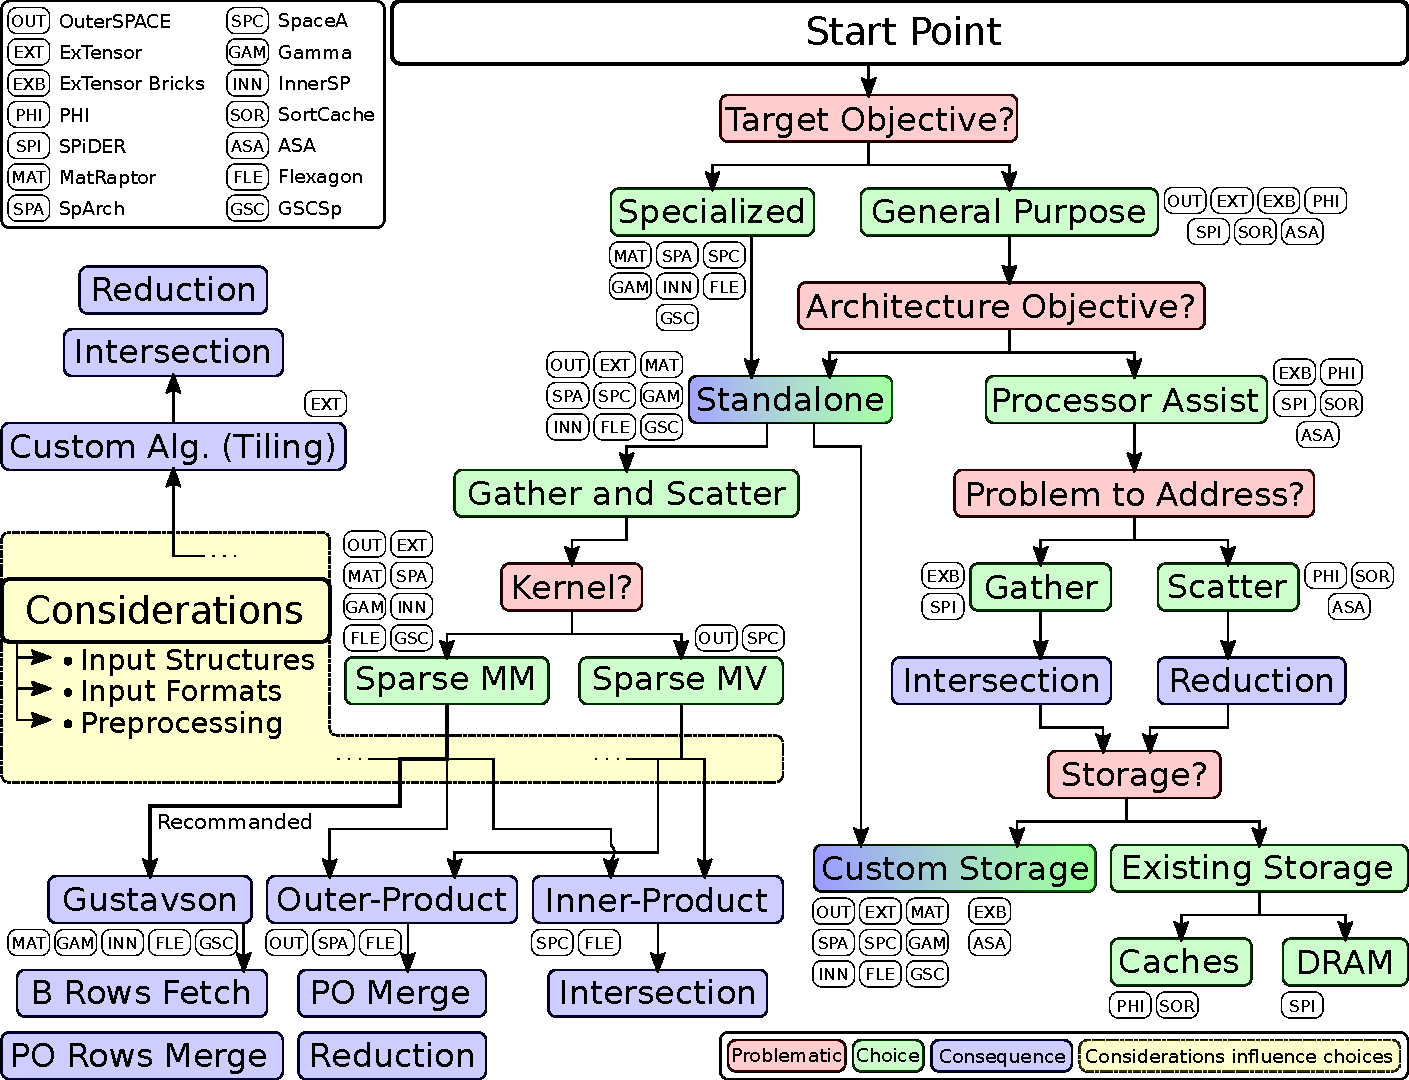
\includegraphics[width=\linewidth]{Chapter_SoA/Figures/PDF/Taxonomy.pdf}
    \caption{Flow Diagram for Architecture Selection}
    \label{fig:soa:taxonomy}
\end{figure}

There is no single "best overall" accelerator. A designer must consider the required performance, the available area and the class of problems to be addressed. In Figure~\ref{fig:soa:taxonomy} we present a flow diagram which can guide a designer towards an architecture based on their requirements. Starting from the top-right of the figure, the designer must first decide between a \emph{specialized accelerator} for a specific kernel or a \emph{general purpose accelerator}. The former is preferable if performance must be maximized, requiring a \emph{standalone} accelerator addressing both \emph{gather} and \emph{scatter} (\emph{e.g.} MatRaptor, SpArch, Gamma and InnerSP).

A \emph{general purpose accelerator} can either take the form of a highly configurable \emph{standalone} block (\emph{e.g.} OuterSPACE and ExTensor) or a \emph{processor assist} that boosts performance for a specific task. With a \emph{processor assist} (rightmost branch in the figure), the processor still performs important parts of the kernel, typically the multiplications, but off-loads the \emph{scatter} or \emph{gather} tasks to the accelerator, as these are the tasks which are the bottleneck with a traditional cache hierarchy. For example, for an \algo{IP} algorithm, the difficult part of the \emph{gather} task is performing the \emph{intersection} (e.g. the ExTensor bricks and SPiDRE).  Conversely, with \algo{OP} or \algo{Gust}, the challenge with the \emph{scatter} is to efficiently perform \emph{reductions} (e.g. PHI, SortCache and ASA). Finally, the designer must decide whether the storage is done by reusing existing memory resources (\emph{e.g.} PHI, SPiDRE and SortCache) or through custom caches/memories.

Going back to the case of a \emph{standalone} accelerator, the algorithms differ according to the supported kernels. For sparse MV, the accelerators studied here have opted for an \algo{OP} algorithm. For sparse MM, the designers of three of the five highest performing accelerators have chosen \algo{Gust} algorithm, as this algorithm provides a good trade-off, simplifying the \emph{gather} by reusing input $B$-rows and the row-by-row generation of the output, simplifying the \emph{scatter} aspect. The fact that the outputs are generated row-by-row, facilitates parallel implementations. \algo{Gust} works well with \emph{(UOP, CP)}, providing consistent input and output formats. Beyond the basic algorithm, \emph{tiling} approaches, as proposed by ExTensor, can be explored.

Orthogonal to previous choices, other design considerations are important. First, the starting point needs to be defined: some accelerators require software to perform \emph{tiling} (\emph{e.g.} ExTensor) or to rearrange the rows to improve performance (\emph{e.g.} Gamma). The cost of such preprocessing can be high, and is usually only justified if the same matrix is reused multiple times.